\subsection{Постановка задачи на разработку программы}
    Цель работы - реализовать систему скелетной анимации.

\bigskip
Основные задачи работы:

\smallskip
\begin{my_enumerate}
\item Создание исходных данных (файлов) для скелетной анимации.
\item Загрузка анимации из файла (содержание описанно в ТЗ).
\item Рассчет кадров анимации.
\item Воспроизведение анимации на экране средствами OpenGL.
\end{my_enumerate}

Второстепенные задачи работы:
\begin{my_enumerate}
\item Предоставление пользователю возможности перейти к любому моменту времени в анимации.
\item Отрисовка костей модели.
\item Возможность вкл./выкл. учет нормалей и материалов во время отрисовки.
\item Поддержка двух видов камер в OpenGL. Первый вид это камера, движение которой сковано орбитой вокруг модели, и другой тип это камера двигающаяся совершенно свободно.
\end{my_enumerate}


\subsection{Описание алгоритма и функционирования программы}


%=============================================================
\subsubsection{Выбор алгоритма}

\paragraph{Различные подходы}
к созданию систем 3-х мерной анимации балансируют между методами с большим количеством вычислений и методами, требующими большого объема памяти. Условно можно выделить явные и неявные системы анимации.

\paragraph{Явные системы анимации} хранят отдельную модель для каждого кадра.
После записи данных в файл, существует много методов для воспроизведения анимации.
Такие методы требуют лишь элементарной математики.
Однако типичная запись одного трэка анимации для одного персонажа занимает около 10MB (в формате MD3).

\begin{figure}[h!]
    \centering
    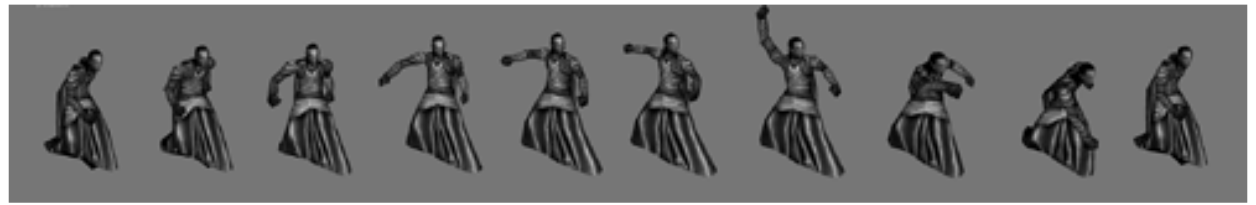
\includegraphics[width=0.8\textwidth]{explicit_animation.png}
    \caption{Каждому кадру соответствует своя модель}
\end{figure}

Предпочтение явным системам отдается, когда необходимо анимировать большие группы людей или животных.

\paragraph{Неявные системы анимации} хранят не модели, а более высокоуровневое описание движения.
В частности неявные \textbf{системы скелетной анимации} содержат описание (через матрицу поворота) для каждой кости, как например локоть, плечо, шея.
В реальном времени эти описания применяются к неанимированной модели для рассчета следующего кадра анимации.
Эти рассчеты обычно требуют сложной математики с матрицами и тригонометрией.
А следовательно и много CPU времени.


\begin{figure}[h!]
    \centering
    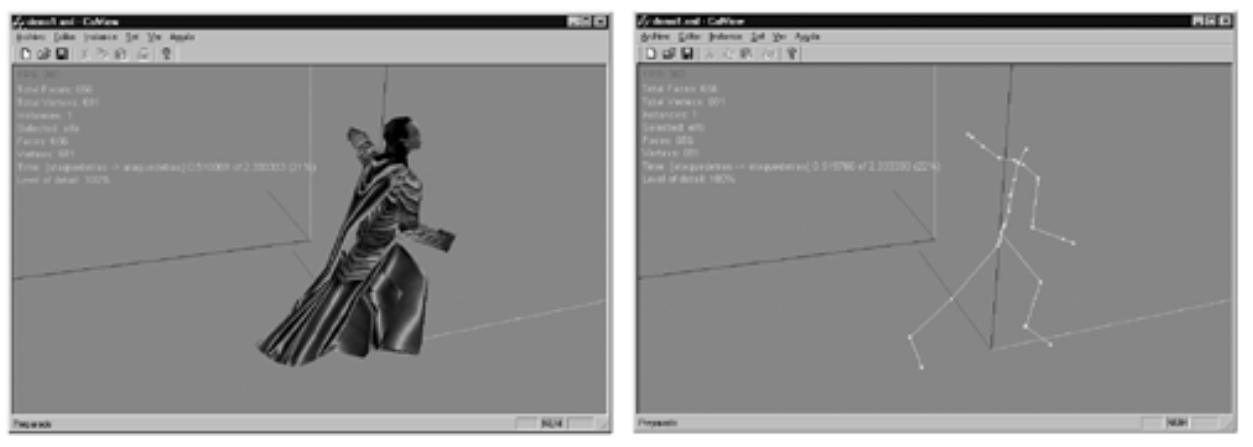
\includegraphics[width=0.8\textwidth]{implicit_animation.png}
    \caption{\scriptsize{Слева: анимированный персонаж; справа: скелет для данного кадра}}
    %\label{fig:awesome_image}
\end{figure}

Неявные системы используются, когда действия персонажа связанны с другими предметами и нельзя предугадать все возможные варианты анимации.
Например для того, чтобы ставить ступню параллельно поверхности при движении по неровной земле.


%=============================================================
\subsubsection{Описание алгоритма и структур данных}
Для реализации требуются 3 вещи: 
\begin{description}
\item[Скелет] Скелет определяет иерархию частей тела персонажа. 
Скелет, - это дерево из костей.

\item[Трэк анимации] В трэке содержатся матрицы поворота скелета в ключевые моменты времени.
Трэк, - это массив пар (время, набор матриц поворота).

\item[Модель]  - это полигональная модель.
\end{description}

Для создания эффекта анимации необходимо извлекать из трэка набор матриц поворота соответствующий настоящему моменту времени. Применять этот набор матриц к скелету, а затем применять позу скелета к модели.

\paragraph{Применение описания из трэка к скелету}
Матрицы поворота для всех костей записываются в трэке относительно матрицы поворота родителя.
Поэтому для деформации скелета необходимо применять матрицы последовательно.
Мы начинаем с корневой кости и применяем к ней описанную в трэке анимации матрицу поворота.
Затем, мы двигаемся вглубь скелета применяя матрицу родителя и матрицу описанную в трэке (то есть считаем глобальную матрицу поворота для данной кости), пока не рассмотрим все кости.

\begin{figure}[h!]
    \centering
    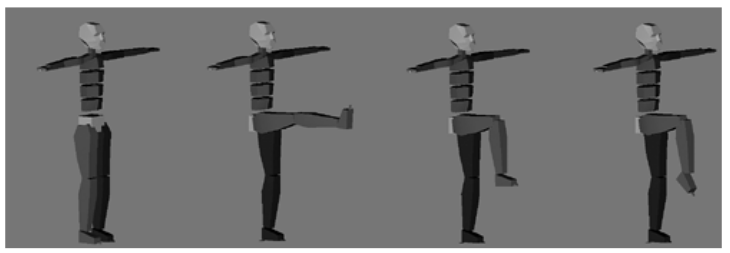
\includegraphics[width=0.8\textwidth]{forward_kinematics.png}
    \caption{\scriptsize{Применение преобразований, начиная от копчика (корневой кости) и заканчивая ступней.}}
    %\label{fig:awesome_image}
\end{figure}

\paragraph{Применение деформации скелета к модели}

После того как рассчитанны матрицы поворотов для скелета, их необходимо применить на вершины модели.
Для этого используется рекурсивный алгоритм очень похожий на предыдущий (п. 3.2.2.1).

\begin{scriptsize}
\begin{verbatim}
deform (bone root, mesh original, mesh deformed)
  for each child_bone of root
    for each vertex in the original mesh
      if bone_weight > 0
          apply bone global transform to vertex
          scale the resulting point by the bone weight
          store the result in deformed
      end if
    end for
    if child_bone has children
      deform (children of this node, mesh original, deformed)
    end if
  end for
\end{verbatim}
\end{scriptsize}


\subsubsection{Реализация системы скелетной анимации}

Для реализации  было созданно несколько функциональных блоков.
Диаграмма основных блоков:

\begin{figure}[h!]
    \centering
    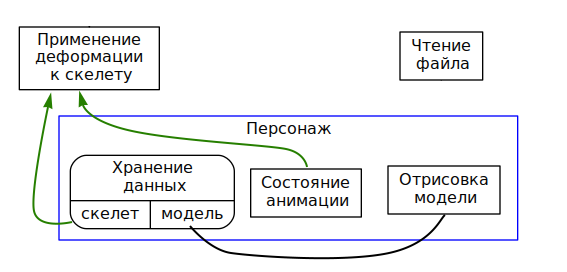
\includegraphics[width=0.8\textwidth]{block_diagram.png}
    \caption{\scriptsize{Схема логических блоков в программе}}
   %\label{fig:awesome_image}
\end{figure}


\paragraph{Описание системы, блок чтения файла}
Заполняет структуры данными из файла.
С помощью библиотеки Assimp производится чтение из файла. Для оптимальной работы данные перераспределяются из структур Assimp в свои. Другие функции этой библиотеки не используются.
Ниже приведен упрощенный код считывающий информацию из файла и строящий стуктуры данных.

\begin{scriptsize}
\begin{figure}
\begin{verbatim}
public void LoadScene(byte[] filedata)
{
    using (MemoryStream fs = new MemoryStream(filedata))
    {
        _cur_scene = new SceneWrapper(ReadAssimpScene(fs, "dae"));
        // у входных данных всегда только один трэк анимации
        _animation_track = _cur_scene.Animations[0];
        // блок применения описаний из трэка анимации к скелету
        _action = new Animator(_animation_track);
        // корневая кость скелета
        BoneNode bones = _cur_scene.BuildBoneNodes("Armature");
        // модель
        Node mesh = _cur_scene.FindNode("Mesh");
        // блок состояния анимации
        ActionState state = new ActionState();
        // блок персонажа
        _enttity = new Entity(_cur_scene, mesh, bones, state);
    }
}
\end{verbatim}
\end{figure}
\end{scriptsize}


\paragraph{Описание системы, блок состояния анимации}
Хранит состояние анимации. Наиболее важные поля:
\begin{itemize}
\item Название трэка анимации.
\item Настоящий момент времени в секундах.
\item Индексы всех ключевых кадров и время каждого ключевого кадра.
\end{itemize}

Есть фyнкция SetTime(\dots) для перехода к определенному моменту времени. Она находит интервал между ключевыми кадрами, подсчитывает величину интерполяции.

\begin{verbatim}
// функция в блоке состояния анимации для прыжка к определенному времени
public void SetTime(double time_seconds)
{            
    double time_ticks = time_seconds * TickPerSec;
    // когда время в секундах переполняеться, запускаем анимацию с начала
    double time = time_ticks % TotalDurationTicks;
    // поиск интервала между ключевыми кадрами
    int start_frame = FindStartFrameAtTime(time_seconds);
    int end_frame = (start_frame + 1) % KeyframeCount;
    // нахождение значения для интерполяции между ключевыми кадрами
    double delta_ticks = KeyframeTimes[end_frame] - KeyframeTimes[start_frame];
    // если начали анимацию заново
    if (delta_ticks < 0.0)
    {
        delta_ticks += TotalDurationTicks;
    }
    double blend = (time - KeyframeTimes[start_frame]) / delta_ticks;
    // приписываем результаты рассчетов
    OriginKeyframe = start_frame;
    TargetKeyframe = end_frame;
    KfBlend = blend;
}
\end{verbatim}



\paragraph{Описание системы, блок хранения данных}
Работает со скелетом и моделью.
Реализует функции поиска костей в скелете или подмоделей в модели.
Функция BuildBones строит скелет по данным из модели (скелет как отдельный класс не существует, он определяеться корневой костью).

Ниже приведен класс описывающий кость скелета:
\begin{verbatim}
class BoneNode
{
    public string Name;
    public Matrix4 GlobalTransform;
    public Matrix4 LocalTransform;

    public BoneNode Parent;
    public List<BoneNode> Children;
    public BoneNode(Node assimp_node) { ... }
}
\end{verbatim}


\paragraph{Описание системы, блок деформации скелета}
Применяет данные, описывающие (в матрицах поворота) новую позицию для каждой кости к костям из скелета.
То есть деформирует скелет в соответствии с моментом времени в анимации. На вход блока подается класс ActionState, содержащий информацию о состоянии анимации и корневая кость скелета.

\begin{verbatim}
// функция для извлечения матриц поворота из трэка и применения их к скелету
public void ChangeLocalFixedDataBlend(ActionState st)
{
    // для каждой кости создает свой канал анимации    
    foreach (NodeAnimationChannel channel in _action.NodeAnimationChannels)
    {
        BoneNode bone_nd = _scene.GetBoneNode(channel.NodeName);
        // поворот кости
        Quaternion target_roto = Quaternion.Identity;
        if (channel.RotationKeyCount > st.TargetKeyframe)
        {
            target_roto = channel.RotationKeys[st.TargetKeyframe].Value.eToOpenTK();
        }
        Quaternion start_frame_roto = channel.RotationKeys[st.OriginKeyframe].Value;
        // интерполяция поворота между двумя ключевыми кадрами
        Quaternion result_roto = Quaternion.Slerp(start_frame_roto, target_roto, (float)st.KfBlend);
        // сдвиг кости
        Vector3 target_trans = Vector3.Zero;
        if (channel.PositionKeyCount > st.TargetKeyframe)
        {
            target_trans = channel.PositionKeys[st.TargetKeyframe].Value;
        }
        Vector3 cur_trans = channel.PositionKeys[st.OriginKeyframe].Value;
        // интерполяция сдвига между двумя ключевыми кадрами
        Vector3 result_trans = cur_trans + Vector3.Multiply(target_trans - cur_trans, (float)st.KfBlend);
        // объединение поворота и сдвига
        Matrix4 result = Matrix4.CreateFromQuaternion(result_roto);
        result.Row3.Xyz = result_trans;
        bone_nd.LocalTransform = result;
    }
}

// функция для рассчета глобальной матрицы поворота для каждой кости
// эта матрица будет позднее применена к вершинам модели
private void ReCalculateGlobalTransform(BoneNode nd)
{
    nd.GlobalTransform = nd.LocalTransform * nd.Parent.GlobalTransform;
    foreach (var child in nd.Children)
    {
        ReCalculateGlobalTransform(child);
    }
}
\end{verbatim}



\paragraph{Описание системы, блоки отрисовки модели}
Загружает данные о модели в OpenGL.
Запрашивает OpenGL об отводе буферов памяти под вершины, нормали, цвета вершин и массив индексов. Применяет свойства материала, например: цвет, коэффициент рассеивания света, коэффициент свечения и т.д.

Данные o вершинах, материалах и нормалях необходимо загружать в буферы памяти расположенные на видеокарте для того что бы обеспечить приложению приемлимую скорость отрисовки.
Ниже приведен код для загрузки данных в память видеокарты:

\begin{verbatim}
// объект содержащий номера буферов в OpenGL
struct Vbo
{
    public int VertexBufferId;
    public int NormalBufferId;
    public int ElementBufferId;
    public int NumIndices;
}

// функция для создания нового буфера 
// и заполнения его данными из массива векторов
private void NewOpenGLBufferWithFloats(out int outGlBufferId, List<Vector3D> dataBuffer) 
{
    GL.GenBuffers(1, out outGlBufferId);
    GL.BindBuffer(BufferTarget.ArrayBuffer, outGlBufferId);
    int sizeof_vec3d = 12; // X,Y,Z = 3 floats, 4 bytes each
    var byteCount = dataBuffer.Count * sizeof_vec3d;
    var temp = new float[byteCount];
    var n = 0;
    foreach(var v in dataBuffer)
    {
        temp[n++] = v.X;
        temp[n++] = v.Y;
        temp[n++] = v.Z;
    }
    GL.BufferData(BufferTarget.ArrayBuffer, (IntPtr)byteCount, temp, BufferUsageHint.StreamDraw);
    VerifyArrayBufferSize(byteCount);
    GL.BindBuffer(BufferTarget.ArrayBuffer, 0);
}

// функция для загрузки данных о модели в память видеокарты
private void Upload(out Vbo vboToFill)
{
    vboToFill = new Vbo();    
    NewOpenGLBufferWithFloats(out vboToFill.VertexBufferId, _mesh.Vertices);
    if (_mesh.HasNormals)
    {
        NewOpenGLBufferWithFloats(out vboToFill.NormalBufferId, _mesh.Normals);
    }
}

\end{verbatim}

Для создания эффекта движения нeобходимо каждый кадр менять содержимое буферов расположыенных на видеокарте.
А именно необходимо менять координаты вершин и направления нормалей к каждой вершине (для корректного отображения света/тени).
Для этого необходимо послать запрос к драйверу OpenGL и получить указатель на память с загруженными ранее данными.
Далее приведен код модифицирущий данные в буфере для следующего кадра.

\begin{verbatim}
// функция в блоке отрисовки модели для получения доступа к буферу OpenGL
public void BeginModifyNormalData(out IntPtr data, out int qty_normals)
{
    GL.BindBuffer(BufferTarget.ArrayBuffer, _vbo.NormalBufferId);
    data = GL.MapBuffer(BufferTarget.ArrayBuffer, BufferAccess.ReadWrite);
    qty_normals = _mesh.Normals.Count;
}
// функция в блоке отрисовки модели для освобождения буфера OpenGL
public void EndModifyNormalData()
{
    bool data_upload_ok = GL.UnmapBuffer(BufferTarget.ArrayBuffer);
    if (! data_upload_ok)
    {
        throw new Exception("OpenGL driver has failed.");
    }
}

// функция в блоке персонажа для применения матриц костей к вершинам модели
public void RecursiveTransformVertices(Node node)
{
    foreach (int mesh in nd.Meshes)
    {
        // получаем указатель на буфер в OpenGL
        IntPtr pbuf_opengl;
        int qty_vertices;
        mesh.BeginModifyVertexData(out pbuf_opengl, out qty_vertices);
        // изначальная модель без деформаций
        Mesh original_data = mesh.OriginalData;
        // go over every vertex in the mesh
        unsafe
        {
            int sz = 3;         // размер шага
            float* coords = (float*)pbuf_opengl;
            for (int vertex_id = 0; vertex_id < qty_vertices; vertex_id++)
            {
                Matrix4 matrix_with_offset = mesh._vertex_id2matrix[vertex_id];
                // получить изначальные координаты вершины
                Vector3 vertex_default = original_data.Vertices[vertex_id];
                Vector3 vertex;
                Vector3.Transform(ref vertex_default, ref matrix_with_offset, out vertex);
                // Применение веса к вершине
                Vector3 delta = vertex_default - vertex;
                vertex += delta *  mesh._vertex_id2bone_weight[vertex_id];
                // Запись новых координат обратно в буфер OpenGL
                coords[vertex_id*sz + 0] = vertex.X;
                coords[vertex_id*sz + 1] = vertex.Y;
                coords[vertex_id*sz + 2] = vertex.Z;
            }
        }
        mesh.EndModifyVertexData();

        foreach (Node child in nd.Children)
        {
            RecursiveTransformVertices(child);
        }
    }
}
\end{verbatim}


\paragraph{Описание системы, блок прерсонажа}
Объединяет компоненты необходимые для анимации одного персонажа. Хранит ссылки на скелет (корневую кость), состояние анимации (ActionState), на саму модель и на класс отрисовки модели (MeshDraw).
    \medskip
    В частности блок персонажа применяет трансформации из скелета к вершинам модели (взвешивая действие каждой кости на вершину) и модифицирует данные в буфере данных OpenGL, что и создает эффект анимации.


\subsection{Mетод организации входных и выходных данных}

\subsubsection{Описание метода входных и выходных данных}
Входными данными является файл в формате collada (.dae)
, в котором в обязательном порядке должны присутствовать следующие элементы:
\begin{my_enumerate}
\item Одна полигональная модель.
\item Один трэк анимации.
\item Один скелет.
\end{my_enumerate}

Если не выполненны условия на наличие полигональной модели,
трэка анимации и связанного с моделью скелета то
у программы не хватит информации для воспроизведения анимации.

Выходными данными является отображение анимации на экране.


\subsection{Выбор состава технических средств}

\subsubsection{Состав технических и програмных средств}
Для возможности запустить приложение необходимо учесть следующие системные требования:
\begin{my_enumerate}
\item Компьютер, оснащенный:
    \begin{my_enumerate}
    \item Обязательно 64-разрядный (x64) процессор с тактовой частотой 1 гигагерц (ГГц) или выше;
    \item 512 мегабайт (ГБ) оперативной памяти (ОЗУ);
    \item 2 ГБ (для 64-разрядной системы) пространства на жестком диске;
    \item графическое устройство OpenGL с драйвером версии 3.1 или выше.
    \end{my_enumerate}
\item Монитор
\item Видеокарта
\item Мышь
\item Клавиатура
\end{my_enumerate}

\bigskip

Также необходимо учесть следующие програмные требования:
\begin{my_enumerate}
\item Поддержка OpenGL версии 3.1
\item 64-битная операционная система Windows 7.
\item .NET Framework версии 4.5.1
\item Библиотека Assimp версии 3.1
\item Библиотека OpenTK версии 1.1.4
\end{my_enumerate}

Программа была протестирована и отлажена на версии OS Windows 7 с использованием .Net Framework 4.5.1, OpenTK версии 1.1.4 и Assimp версии 3.1.

Качество и корректность работы программы при других версиях библиотек и операционных систем не проверялось.

Программа использует буферы графической памяти типа STREAM\_WRITE и функции glMapData и glSubBufferData которые в OpenGL официально поддерживаются лишь с версии 3.1

Технические требования к памяти и периферии не превышают технических требований к операционной системе Windows 7 с установленным на ней .Net Framework 4.5.1
